\documentclass[8pt]{article}

\usepackage{amsmath,amsthm,amssymb,amsfonts,mathrsfs,bbm}
\usepackage{graphicx}
\usepackage[margin=1in]{geometry}

\newcommand{\N}{\mathbb{N}}
\newcommand{\R}{\mathbb{R}}
\newcommand{\Z}{\mathbb{Z}}
\newcommand{\tb}{\textbf}
\newcommand{\tn}{\textnormal}
\newcommand{\ti}{\textit}

\pagestyle{empty}

\begin{document}

\subsection*{Intro}
If programs had to share hardware themselves, very difficult; conflicts easily; interfere with each other, etc.
\\
OS' goal is to run programs easily, effectively, securely etc.
OS also handles concurrency, provides persistence, and supports networking, system security
\\
Process = running program; Program = stored instructions; Address Space = Programs Data;
\\
PCB (Process Control Block) is used to keep track of process info
\\
Every process has a parent; Starts at initial ends in final (zombie) state.
If Parent finishes before child, child becomes orphan and root becomes parent
\\
pid\_t fork() $\rightarrow$ creates copy of current process; continuing at execution from return of fork().
\\
Returns pid of child to parent, 0 to child, and -1 if failed (no child created)
\\
pid\_t wait(int\* w\_status) $\rightarrow$ waits for a child process of the current running process;
\\
Returns pid of child that terminated, w\_status gets filled with info on termination status
\\
If process terminates without parent calling wait(), becomes zombie.
\\
int exec(const char *pathname, char *const argv[]) $\rightarrow$ replaces the current program with a new one, command line arguments being passed in argv.
\\
Returns: On success does not return (nowhere to return to) and runs new program. On fail returns -1
\\
int pipe(int p[2]) $\rightarrow$ creates a communication channel, normally called before fork in order to communicate
\\
Returns: On success returns 0, p[0] is read, p[1] is write. On failure returns -1
\\
int dup(int fd) $\rightarrow$ changes pointer of file descriptor
\\
Returns: On success returns new file descriptor and moves pointer. On failure returns -1
\subsection*{Schedulers}
User mode versus Kernel Mode: User mode does not have access to read/write I/O devices, or use memeory outside its space, Kernel mode has full access;
In order to use I/O as user, use system call, causes a trap;
\\
Time-sharing $\rightarrow$ multiple processes run together on a single machine as though they are in sole control
multiprogramming - when process waiting for I/O, OS can have another process use CPU
\\
multitasking - each process gets a time slice, a time limit before being forced off CPU
\\
Time needed by CPU for process is job or CPU burst; time to wait is an I/O burst
\\
preempting = swapping before process is done
\\
$T_{turnaround} = T_{completion} - T_{arrival}; T_{response} = T_{firstrun} - T_{arrival}$
\\
FIFO = First In First Out $\rightarrow$ easy to implement (simple queue), no preemption, not very good. Relies on arrival order
\\
SJF = Shortest Job First $\rightarrow$ priority queue based off job length, no preemption, optimal average turnaround when arriving at same time. Relies on arrival order
\\
STCF = Shortest Time-to-Completion First $\rightarrow$ priority queue based off job length, preempts if job appears with shorter time left. Short jobs don't have to wait for long jobs. Can still be bad and starve with long jobs / lots of short jobs
\\
SJF and STCF require an oracle $\rightarrow$ a way to decide how long jobs take
\\
RR = Round Robin $\rightarrow$ FIFO queue, Preemption as each job gets single time slice, Low response time, High turnaround time.
\\
Multi Level Queue $\rightarrow$ Process that need fast response but little CPU should be highest, Process that need long CPU and little I/O lowest priority
Ruleset:
1) If Priority(A) $>$ Priority(B); A runs,\\
2) If Priority(A) $=$ Priority(B); A\&B run in RR using time slice of given queue,\\
3) When process enters it starts at highest priority $\rightarrow$ Feedback\\
4) Once a process has used its time slice its priority gets reduced $\rightarrow$ Confront gaming the system and adding feedback\\
5) After some time period S, move all processes to topmost queue $\rightarrow$ Priority Boost\\
\\
Lottery $\rightarrow$ each process gets tickets, scheduler randomly picks a ticket at each time slice, that process gets the time slice. Can gift tickets
out inversely to completion time, nondeterministic, no job can be starved, a short job can get unlucky. Fair in long term, stateless.
\\
Stride Scheduling $\rightarrow$ deterministic but with same fairness as lottery. Fair in short and long term. Requires state
\\
Linux $\rightarrow$ sched\_latency (time period for all runnable processes once.), divided into n slices where n is the number of processes. min\_granularity is the minimum size of time slice.
For each slice picks the process with the smallest runtime that still needs to run. Uses priority system with niceness (high nice $=$ lower priority).
Updates time slice to worry about priority. vruntime k = vruntime k + runtime * weight 0 / weight k. uses states. new process is set to the shorted vruntime
of the existing processes. small vruntime $=$ larger weight $=$ longer physical runtime. uses red-black tree for balancing.
\subsection*{Memory}
Single Programming: splits memory between OS and user process. Addresses assigned at compile time (not used in modern computers)
Multi Programming: Processes have to share main memory; Simple solution is to assign contiguous memory for each process.
Memory actually gets fragmented and split, may even have to use disk
Programmers view: Program Code @ 0 (static values as well), Heap starts at top and goes down, Stack starts at bottom and moves up. Heap = malloc, stack = declaration
Memory virtualization gets from messy fragmentation to programmer view.
32 bit = 4 GB of memory. Registers, instructions, address bus and data bus $=$ one word. Word size dependent on architecture, usually a power of 2.
\\
How? limited direct execution but since it happens at every stage also hardware-based address translation. Loader may statically translate before execution
$$physical address = virutal address + base$$ where $base$ is start of process. $bounds$ maximum address. bounds may be used on vr or pr.
MMU = Memory Management Unit; hardware responsible for all memory translation. part of the CPU but sits between core and address bus.
Problems with base and bounds is that if memory needs to grow, lots to update.
We want sparse address space, segemenation is how we get that. parts are independent. Divided into 3 segments; Code, Heap, Stack.
Last 3 bytes are offset, first 2 bits are segment bits. \\
allows for change in how it grows and where, etc. Can also allow for sharing of memory if read only\\
Can result in external fragmentation, need to compact in order to reclaim.
\\
Page table, uses valid bit to show if that entry is valid (not all memory needs allocated), converts VPN to PFN
If total address space is $2^m$ bytes and page size is $2^n$ then VPN is $m-n$ bits and offset is $n$ bits
If physical memory is $2^m$ bytes and (frame) page size is $2^n$ then PFN is $m-n$ bits and offset is $n$ bits
Thus PhysAddr = PFN $\times$ frame\_size $+$ offset
\\
Example:
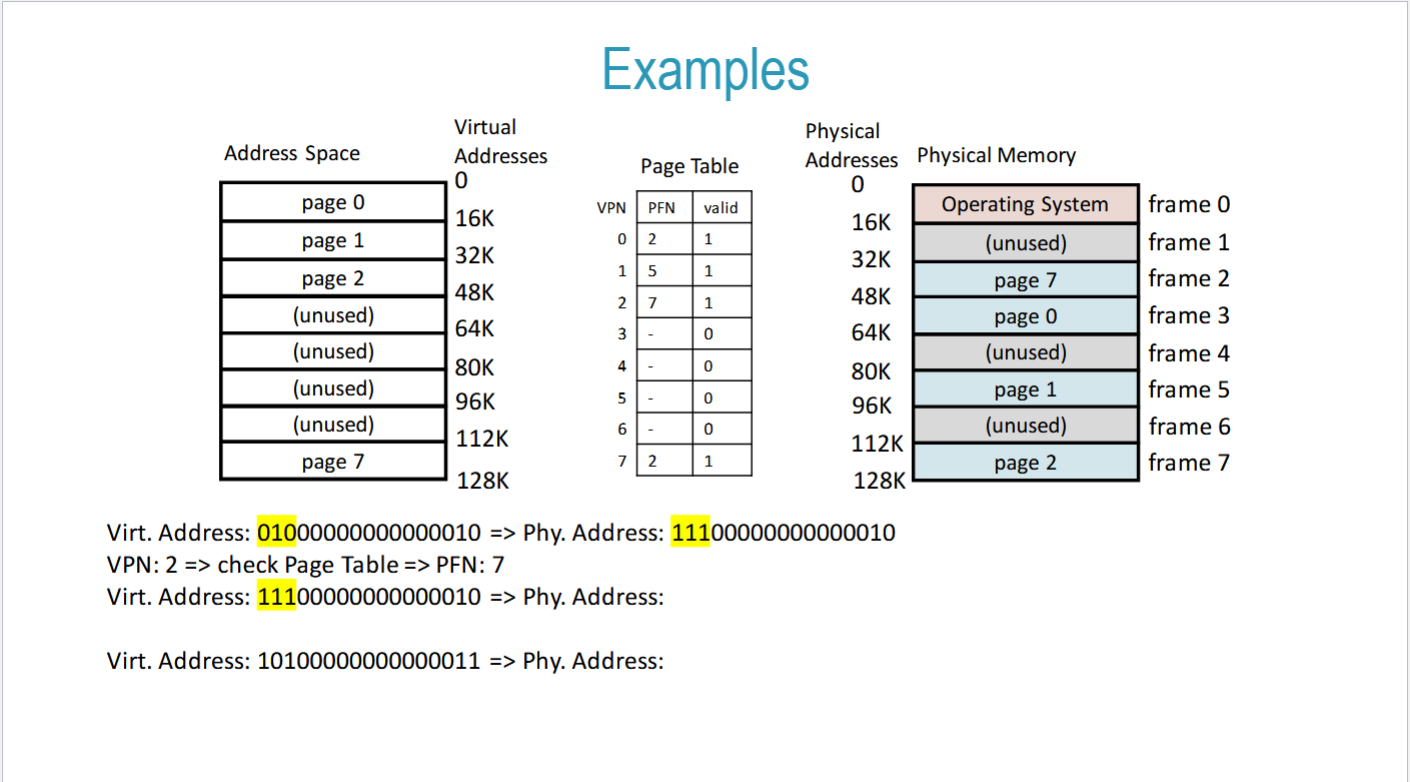
\includegraphics[scale=0.25]{VirtualMemoryExample1.png}
Linux page size is 8KB, Linux also uses mutli level structure, lookup is slow though
\\
TLB = cache for page table entries. May use LRU (least recently used) or Random for misses. context switches make misses more often.
\\
Page table includes present bit, to state if in physical memory or swap (disc). Page fault occurs when attempting to access page not in memory
\\
Cache styles:\\
FIFO $\rightarrow$ easy to implement and exactly as sounds, can lead to Beladys anomly in which larger cache leads to worse response
\\
Random $\rightarrow$ as it sounds; LRU $\rightarrow$ better than FIFO, no anamoly, slow.
\\
Thrashing is when a process spends more time on page-fault than executing.
\subsection*{Concurrency}
Threads are multiple points of execution of a program within a single process. Needs a TCB to keep track. Threads share data and heap.
Lower cost to create and switch context. Can switch at any instruction
\\
Race condition bug - may have threads stepping over one another leading to undesirable affects.
\\
Locks provide mutual exclusion to a critical section of code.
\\
\end{document}
Process
\\
Program
A static instruction set
\\
Process
A running program
\\
Address space
A set of memory for any non static variables in the program
\\
Program counter
An indication of the current instruction to run
\\
CPU registers
Memory in the CPU for the process to use
\\
Stack pointer
Pointer to the top of the stack, where variables are placed from the process
\\
PCB (Process control block)
A structure outside of the process for the OS to keep track of all the information regarding the process such as address space, registers, program counter, etc.
\\
Scheduler
The OS / hardware necessary to decide which process to run and when
\\
Running (state)
Process is currently using the CPU, registers
\\
Ready (state)
Process is ready to run
\\
Blocked (state)
Process is waiting for I/O
\\
Context Switch
Anytime the CPU changes process
\\
Parent (process)
A process that has children (from a fork command)
\\
Child (process)
A process called from a fork command, has a parent
\\
Zombie (process)
A process that terminated without wait being called in the parent
\\
Orphan (process)
A child process that finishes after the parent
Process System calls (FORK, EXEC, WAIT, PIPE, DUP)
\\
Fork $\rightarrow$ initiates a new child process from the line after the fork command. Returns pid of child to parent, 0 to child, and -1 if failed
\\
Exec $\rightarrow$ runs a different program. Does not return if successful, returns -1 if failed
\\
Wait(int * w\_status) $\rightarrow$ called by a parent to wait for some child process to finish. Returns child pid and houses the status of execution in w\_status
\\
pipe $\rightarrow$ initializes a pipe to be used by two different programs to allow information to be passed. Returns -1 on fail.
\\
dup $\rightarrow$ changes where the file descriptor points. Returns -1 on fail.
\\
Pipes
A pipe allows communication between processes. Reads from p[0] and writes to p[1].
\\
Time-sharing
multiple processes run together on a single machine as though they are in sole control
\\
Multiprogramming
when process waiting for I/O, OS can have another process use CPU
\\
Multitasking
each process gets a time slice, a time limit before being forced off CPU
\\
User mode (CPU)
does not have access to read/write I/O devices, or use memory outside its space,
\\
Kernel mode (CPU)
Has full access to read/write I/0 devices, and use any memory in the computer
\\
Privileged instruction
These are the intructions that user mode can not call
\\
System call
A way for user mode to initiate a priviledged instruction
\\
Trap
System calls cause a trap which the OS handles, doing the instruction most likely, and then goes back to User Mode
\\
Job (or CPU burst)
The amount of time a process needs from the CPU
\\
I/O burst
The amount of time a process needs for I/O
\\
CPU Bound
A process that has a lot of CPU burst time
\\
I/O Bound
A process that requires a lot of I/O time
\\
Preemption
The notion in scheduling when a context switch will happen without a process finishing
\\
Turnaround time
$T_{completion} - T_{arrival}$
\\
Response time
$T_{first\_response}-T_{arrival}$
\\
FIFO
First In First Out: Simple, no preemption, relies on arrival time
\\
SJF
Shortest Job First: priority queue based off completion time, based on arrival time
\\
STCF
Shortest Time-to-Completion First: priority queue based off time to finish, will preempt if another job shows up with shorter time to completion. Can starve long jobs
\\
RR
Round Robin: Optimal Response time, will simply cycle each process through a time slice of a certain size. Does not give any priority
\\
Lottery
Each process gets a random amount of tickets (can be inveresly proportional to completion time) that the OS then picks a random ticket and gives that process the time slice
\\
Stride
Deterministic solution to lottery, requires states, gives each process a stride amount based off time to finish. grabs the process with the smallest stride and increments the process\' pass count by the stride of the process.
\\
MLFQ
Multi Level Fair Queue:
1) If Priority(A) $>$ Priority(B); A runs,\\
2) If Priority(A) $=$ Priority(B); A\&B run in RR using time slice of given queue,\\
3) When process enters it starts at highest priority $\rightarrow$ Feedback\\
4) Once a process has used its time slice its priority gets reduced $\rightarrow$ Confront gaming the system and adding feedback\\
5) After some time period S, move all processes to topmost queue $\rightarrow$ Priority Boost\\
\\
CFS
Linux Scheduler: uses sched\_latency (amount of ms for all processes to run), min\_granularity (min amount of time for one process to run), n (number of process),
nice score (more nice $=$ less weight) to decide that time slice k $=$ sched\_latency * weight k / (weight 0 + weight 1 + $\cdots$ + weight n-1) and
vruntime k = vruntime k + runtime * weight 0 / weight k; thus vruntime is counted less per shed\_latency with higher weight even if physical runtime is longer. Uses red black tree to self balence, and any new process gets the smallest vruntime of any of the existing processes
\\
Time-slice (quanta in RR)
The amount of time for each process to run before a context switch
\\
Oracle (requirement to see into the future)
Used by SJF and STCF to decide the future runtime of the process, and CFS
\\
Tickets (Lottery)
How the OS decides what process to use
\\
Starvation
If a process does not get to run. STCF leads to starvation, FIFO can in rare cases, Lottery can in rare cases
\\
Priority boost (MLFQ)
After S time, return all processes to the highest priority
\\
Virtual runtime (CFS)
The actual time counted instead of physical runtime
\\
Nice value (CFS)
Higher nice is lower weight
\\
Address space (virtual)
The address of the memory in the program (not the actual memory location)
\\
Physical memory
The actual address of the memory in the program
\\
Program code
A section of memory for the instructions and any static variables
\\
Heap
A section of memory for allocated variables (malloc())
\\
Stack
A section of memory for initialized variables (int x;)
\\
Memory virtualization
The process of transforming messy physical memory into pure virtual memory
\\
Virtual address
The not real address of the information
\\
Physical address
The address in the hardware of the information
\\
Address translation
The process of changing a virtual address to a physical address
\\
Base and Bound
Base = the start of the physical address location, bound = max address location, can be virtual or phyiscal. A problem is that if a program needs to use more memory than originally allocated, a lot of updates need to be done.
\\
MMU (Memory Management Unit)
The part of hardware responsible for address translation
\\
Segmentation
The act of splitting physical memory between multiple sections and/or pages, not making one continguous slot of memory
\\
Segment (address space)
Independent parts of the segmentation of physical memory, normally made into a page
\\
Segmentation fault
Attempting to access memory in user mode that the user does not have access to
\\
Sparse address space
A mostly unused address space
\\
Extern fragmentation
Gaps in the segmentation that are not used and unable to fit a full segment
\\
Internal fragmentation
Unused memory that is allocated by an allocator
\\
Compaction
The process to fix fragmentation. Very expensive
\\
Best fit (free-space management policy)
A way to decide how to fill segements, will look for the smallest one that still meets the memory requirement.
\\
Paging (memory)
A process of creating fixed space units for memory
\\
Page table
A table that converts virtual memory to specific pages in memory
\\
Page table entry
A line item that houses the VPN, PFN, and valid bit
\\
Page
A fixed size of memory
\\
Frame
The physical space for a page of memory
\\
VPN (virtual page number)
If total address is $2^m$ and page size is $2^n$ VPN is $m-n$ bits, which describes what page number the address is at
\\
PFN (physical frame number)
If total address is $2^m$ and frame size is $2^n$ PFN is $m-n$ bits, which describes what frame number the address is at
\\
Offset (from start of page)
The rest of the bits used to find that exact section of memory
\\
Physical address = virtual address + offset
\\
Valid bit (page table)
A bit stating if the memory in the page table is able to be used (may not be all of the memory)
\\
TLB (Translation-Lookaside Buffer)
A cache of page table lookups to makes address translation much faster
\\
TLB hit
When the TLB has the lookup already in the cache
\\
TLB miss
When the TLB does not have the lookup and so then much pull it from memory
\\
TLB cache entry
A line in the TLB that translates VPN to PFN, along with a valid bit
\\
Valid bit (TLB cache entry)
Shows if the cache line is valid, does not say anything about the page table entry valid bit
\\
Spatial locality
Memory access is likely to be near other memory accessed
\\
Temporal locality
Addresses are likely to be repeated in time
\\
Memory hierarchy
Registers, L1, L2, L3, RAM. The division of memory into specific areas depending on how likely it is needed
\\
Swap space
The disk, not current working memory that is divided into blocks for one page
\\
Block (swap on disk)
A segment of memory to house one page
\\
Present bit (swap)
If the current page is in memory (1) or on disk (0)
\\
Cache hit
If the TLB or other cache has the asked for information in cache
\\
Cache miss
If the cache does not have the asked for information in cache
\\
Page fault
When the page asked for is not present
\\
High watermark
The amount of free memory to stop swapping from low watermark
\\
Low watermark
The minimum amount of free memory, if under will start pushing pages to swap space
\\
Reference string
A sequence of attempted accesses to model their accesses in different replacement policies
\\
OPT (optimal)
The optimal cache removal based off the reference string
\\
FIFO (first in first out)
As it sounds, the first one in is the first one out on a miss with no free space
\\
Random
Randomly pick a entry for each miss with no free space
\\
LRU (least-recently used)
Remove the least recently used when a miss with no free space
\\
Clock Algorithm
An attempted LRU without lookups to see which was last used. Add a "use bit" to each entry of the cache. Set 1 when line is used. round robin, setting to 0 when 1 is found, otherwise removing the first 0
\\
Belady’s Anomaly
How in FIFO there are cases when larger cache means more misses
\\
Dirty bit (swap)
A bit that starts at 0 and is set to 1 on a write, to know if the page needs to go to swap or not
\\
Thrashing
When there is more time spent on page-faults than execution
\\
Threads
Multiple points of execution of a program within a single process, shares data and a heap with other processes
\\
TCB (Thread Control Block)
A structure for the OS to keep track of different threads
\\
Concurrency vs Parallelism
Concurrency is running one after another on one CPU, parallelism is running items at the same time on different cores
\\
Race condition
When two or more threads step on each other leading to undesireable or weird effects
\\
POSIX
Portable Operating System Inferface, standards for OS APIs
\\
pthreads
a specific api for thread creation and synchronization
\\
pthread\_create(pthread\_t *thread, const pthread\_attr\_t attr, void *(*start\_routine) (void*), void* arg)
Creates a new thread with thread pointing to a buffer to store the id of the new thread, attr describes the attributes of the new thread, starts by invoking start\_routine arg is a pointer to arguments for start\_routine. Returns 0 on success, errror number on error
\\
pthread\_exit()
Terminates calling thread
\\
pthread\_join(pthread\_t th, void **retval)
Wait for a thread to terminate and will add the exit status to the location at retval if not null. 0 on success, error number on error. also deallocates TCB of whatever thread terminated
\\
pthread\_mutex\_lock(pthread\_mutex\_t * mutex, const pthread\_mutexattr\_t * mutexattr)
initalizes a mutex lock, mutex points to the lock, second attribute describes the lock, returns 0 on succcess, error number otherwise
\\
pthread\_mutex\_unlock(pthread\_mutex\_t *mutex)
destroys the mutex, attempting to destroy locked mutex results in undefined behavior
\\
Mutual exclusion
Only one thread at a time
\\
test-and-set
A process of determing if a lock is locked or unlocked by testing the value of a pointer, and setting it to a new value
\\
Spin lock
A system of waiting for a lock to unlock with a while(locked) ;
\\
Spinning loops
What is imployed in a spin lock
\\
pthread\_cond\_wait(pthread\_cond\_t *c, pthread\_mutex\_t *m)
waits for signal to condition c, releases m in while waiting
\\
pthread\_cond\_signal(pthread\_cond\_t *c)
Signals on the condition, waking waiting threads
\\
Producer/consumer (bounded buffer) problem
Consider 2 conumers and 1 producer. Producer puts one 1, then signals that item has been placed. If solved incorrectly both c1 and c2 will attempt to get, causing an error. p1 could also attempt to put on a full buffer.
Fix is to signal both empty and full.
\\
Semaphore
Provides both locking and signaling
\\
sem\_init(sem\_t *s, attr, num of resources)
must init with number of resources, generates a new semaphore at s with attributes and number of resources as described.
\\
sem\_wait(sem\_t *s)
will wait until s has at least 1 resource
\\
sem\_post(sem\_t *s)
will free up one resource of s
\\
Binary semaphore
Using semaphore as locks, having only two states, locked and unlocked. thus binary.
\\
Reader-Writers problem
Multiple people can read from data at one time, but only one writer can write with no readers allowed.
